% !TeX program = pdflatex
% Compile:  tectonic report.tex          (or pdflatex report.tex, twice)
\documentclass[11pt]{article}

\usepackage[margin=1in]{geometry}
\usepackage{microtype, parskip}
\usepackage{amsmath, amssymb, mathtools}
\usepackage{booktabs, siunitx}
\usepackage{caption, subcaption}
\usepackage{xcolor}
\usepackage[hyphens]{url}
\usepackage[hidelinks]{hyperref}
\usepackage{tikz}
\usetikzlibrary{positioning, arrows.meta, calc, shapes.geometric, fit, backgrounds}
\usepackage{graphicx}
\usepackage{listings}

\Urlmuskip=0mu plus 1mu\relax

\lstset{
  basicstyle=\ttfamily\footnotesize,
  breaklines=true,
  showstringspaces=false,
  backgroundcolor=\color{black!4},
  frame=single, framerule=0pt,
  xleftmargin=4pt, xrightmargin=4pt,
}

\newcommand{\PVAF}{\mathrm{PVAF}}
\newcommand{\SSE}{\mathrm{SS_{explained}}}
\newcommand{\SST}{\mathrm{SS_{total}}}
\newcommand{\SSR}{\mathrm{SS_{resid}}}
\newcommand{\Hilbert}{\mathcal{H}}

\title{\bfseries Percent variance accounted for (PVAF) of head motion\\
by the gastric rhythm}
\author{}
\date{}

\begin{document}
\maketitle

\section{Introduction}

The goal of this analysis is to quantify what fraction of the
head-motion power can be linearly accounted for by the gastric rhythm.
The reported quantity is the \emph{percent variance accounted for}
(PVAF) of a head-motion time course $y(t)$ by a small set of regressors
built from the gastric signal. PVAF is reported against three explicit
denominators:

\begin{enumerate}
\item Total head-motion power: the raw 6 degree-of-freedom (dof) motion
time courses with no filtering applied.
\item Head-motion power inside the conventional resting-state
functional MRI (rsfMRI) band, $0.01$--$0.10$~Hz (a standard frequency
range used in resting-state fMRI denoising).
\item Head-motion power inside the narrow gastric band, defined as the
subject-specific gastric peak frequency $\pm 0.015$~Hz.
\end{enumerate}

Two related coupling measures used elsewhere in the project, the
phase-locking value (PLV) and its amplitude-weighted variant (awPLV),
are computed within a single narrow band and are sensitive only to
phase consistency. PVAF places the same coupling on an absolute
variance scale and can be quoted against any frequency window, so it is
the measure used here.

The implementation is in \texttt{pvaf\_total\_motion.py}; the generated
tables and figures are written to \texttt{outputs/}.

\section{Pipeline}

\begin{figure}[h!]
\centering
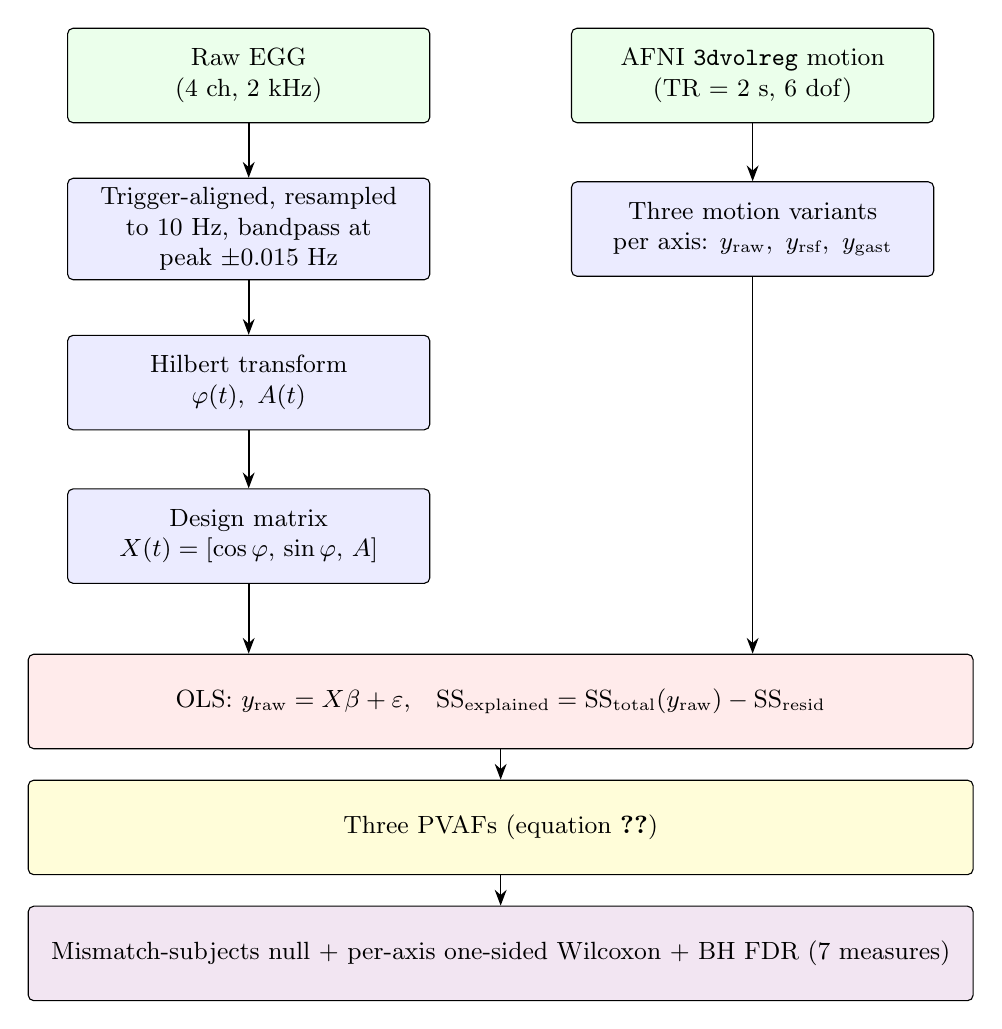
\begin{tikzpicture}[
  x=1cm, y=1cm,
  block/.style={rectangle, draw, fill=blue!8, rounded corners=2pt,
                minimum height=12mm, minimum width=46mm, align=center,
                font=\small},
  data/.style={rectangle, draw, fill=green!8, rounded corners=2pt,
               minimum height=12mm, minimum width=46mm, align=center,
               font=\small},
  wide/.style={rectangle, draw, rounded corners=2pt,
               minimum height=12mm, minimum width=120mm, align=center,
               font=\small},
  arrow/.style={-Stealth, semithick},
]

% Top row: data inputs
\node[data] at (-3.2, 0)   (egg)    {Raw EGG\\(4 ch, 2 kHz)};
\node[data] at ( 3.2, 0)   (motion) {AFNI \texttt{3dvolreg} motion\\(TR = 2 s, 6 dof)};

% Second row: preprocessing
\node[block] at (-3.2, -1.95) (egg_bp)       {Trigger-aligned, resampled\\to 10 Hz, bandpass at\\peak $\pm 0.015$~Hz};
\node[block] at ( 3.2, -1.95) (motion_split) {Three motion variants\\per axis: $y_{\text{raw}},\ y_{\text{rsf}},\ y_{\text{gast}}$};

% Left column (EGG) continues
\node[block] at (-3.2, -3.9) (hilbert) {Hilbert transform\\$\varphi(t),\ A(t)$};
\node[block] at (-3.2, -5.85) (design)  {Design matrix\\$X(t)=[\cos\varphi,\,\sin\varphi,\,A]$};

% Wide rows
\node[wide, fill=red!8]     at (0, -7.95)  (ols)   {OLS: $y_{\text{raw}}=X\beta+\varepsilon$,\quad
  $\SSE = \SST(y_{\text{raw}})-\SSR$};
\node[wide, fill=yellow!15] at (0, -9.55)  (pvafs) {Three PVAFs (equation~\ref{eq:pvaf})};
\node[wide, fill=violet!10] at (0, -11.15) (null)  {Mismatch-subjects null + per-axis one-sided Wilcoxon + BH FDR (7 measures)};

% Arrows: top column flows
\draw[arrow] (egg)     -- (egg_bp);
\draw[arrow] (motion)  -- (motion_split);
\draw[arrow] (egg_bp)  -- (hilbert);
\draw[arrow] (hilbert) -- (design);

% Vertical drops into the wide OLS block
\draw[arrow] (design.south)       -- (design.south       |- ols.north);
\draw[arrow] (motion_split.south) -- (motion_split.south |- ols.north);

% Wide-row flow
\draw[arrow] (ols)   -- (pvafs);
\draw[arrow] (pvafs) -- (null);
\end{tikzpicture}
\caption{Per-run pipeline. Green = data, blue = computational steps; the
three wide blocks below are the single Ordinary Least Squares OLS step (red), the resulting
three PVAF expressions (yellow), and the group-level inference (purple).
The two left-column outputs ($X$ and $y_{\text{raw}}$, the latter inside
\texttt{motion\_split}) feed into the same OLS; that single fit produces
the $\SSE$ that appears in the numerator of every PVAF in
equation~\ref{eq:pvaf}.}
\label{fig:pipeline}
\end{figure}

\clearpage

\section{Data}

\begin{itemize}
\item 84 resting-state runs from 43 healthy adults, re-analysed from the
dataset shared by Levakov, Ganor \& Avidan (2023). Concurrent BIOPAC
cutaneous electrogastrogram (EGG) on the epigastrium and Philips 3T
blood-oxygen-level-dependent functional MRI (BOLD-fMRI) at repetition
time TR = \SI{2}{\second}.
\item Six rigid-body realignment parameters per run from AFNI
\verb|3dvolreg|; files of the form
\path{BIDS_data/sub_motion_files/sub-XX_dfile.r0R.1D}.
\item EGG already preprocessed (trigger-aligned, resampled to
\SI{10}{\hertz}, bandpass at the subject-specific gastric peak
$\pm 0.015$~Hz); files \texttt{gast\_data\_*.npy} and the companion
peak-frequency file \texttt{max\_freq*.npy} live under
\path{derivatives/brain_gast/}, one folder per (subject, run). The peak
frequency typically ranges $0.041$--$0.062$~Hz across subjects.
\item The bandpassed EGG is resampled from \SI{10}{\hertz} to
\SI{0.5}{\hertz} to match the motion grid; both series are then
truncated to the shorter of the two.
\end{itemize}

The six motion columns are read in the order in which they appear in
the AFNI 1D file and are labelled, following the project's existing
convention,
\texttt{[trans\_x, trans\_y, trans\_z, rot\_x, rot\_y, rot\_z]}. The
median PVAF reported across the six axes does not depend on the
ordering of the labels.

\section{Method}

\subsection{Gastric regressors}

The gastric regressor matrix is built once per (subject, run) in three
steps:
\begin{enumerate}
\item Start from the already bandpassed dominant-channel EGG (at
$\SI{10}{\hertz}$). Resample to $f_s = \SI{0.5}{\hertz}$ to match the
motion grid (TR = 2~s).
\item Take the Hilbert transform to obtain the instantaneous phase
$\varphi(t)$ and instantaneous amplitude $A(t)$.
\item Form three regressor columns $\cos\varphi(t)$, $\sin\varphi(t)$,
and $A(t)$, and standardise each column to zero mean and unit variance.
\end{enumerate}

The detail is below. Let $g(t)$ be the bandpass-filtered EGG sampled at
$f_s = \SI{0.5}{\hertz}$ (TR = 2~s). Its analytic representation via the
Hilbert transform is
\begin{equation}
z(t) \;=\; g(t) \;+\; j\,\Hilbert[g](t), \qquad
\varphi(t) \;=\; \arg z(t), \qquad
A(t) \;=\; |z(t)|.
\end{equation}
\textit{where:}
\begin{itemize}\setlength{\itemsep}{1pt}
\item $t$ is the discrete time index, running from $0$ to $N-1$ at
sampling frequency $f_s$;
\item $g(t)$ is the bandpassed dominant-channel EGG (arbitrary units
after z-scoring);
\item $j = \sqrt{-1}$ is the imaginary unit;
\item $\Hilbert[\cdot]$ is the Hilbert transform
(\texttt{scipy.signal.hilbert});
\item $z(t)\in\mathbb{C}$ is the analytic signal of $g$ (real part $g$,
imaginary part the quadrature of $g$);
\item $\arg(\cdot)$ returns the complex argument and $|\cdot|$ the
modulus;
\item $\varphi(t)\in(-\pi,\pi]$ is the instantaneous phase of $g$ at
time $t$;
\item $A(t)\geq 0$ is the instantaneous amplitude (envelope) of $g$.
\end{itemize}

The three-column design matrix is
\begin{equation}
X(t) \;=\; \bigl[\,\cos\varphi(t),\ \sin\varphi(t),\ A(t)\,\bigr].
\label{eq:designmatrix}
\end{equation}
Using $\cos\varphi$ and $\sin\varphi$ rather than $g(t)$ directly is the
standard Fisher (1993) circular-regression trick: the linear combination
\begin{equation}
\beta_1\cos\varphi(t) + \beta_2\sin\varphi(t)
\;=\; R\,\cos\!\bigl(\varphi(t) - \delta\bigr),
\quad
R = \sqrt{\beta_1^{2}+\beta_2^{2}},
\quad
\delta = \mathrm{atan2}(\beta_2,\beta_1),
\end{equation}
\textit{where:}
\begin{itemize}\setlength{\itemsep}{1pt}
\item $\beta_1, \beta_2 \in \mathbb{R}$ are the regression coefficients
on $\cos\varphi$ and $\sin\varphi$ respectively, estimated by ordinary
least squares (OLS) from a particular motion axis;
\item $R \geq 0$ is the recovered in-band amplitude
$\sqrt{\beta_1^2 + \beta_2^2}$;
\item $\delta \in (-\pi,\pi]$ is the preferred-phase offset
$\mathrm{atan2}(\beta_2,\beta_1)$ that the data choose for that motion
axis.
\end{itemize}
The two real degrees of freedom in $(\beta_1,\beta_2)$ recover any
$\delta$ and any $R$. The third column $A(t)$ carries slow modulations
of the gastric envelope. Each column $x$ of $X$ is finally
standardised to zero mean and unit variance, i.e.\ replaced by
$(x - \bar x)/\sigma_x$ where $\bar x$ and $\sigma_x$ are the
time-average and time-standard-deviation of that column. This
rescaling makes the OLS coefficients dimensionless and directly
comparable to each other but does not change the coefficient of
determination $R^{2}$.

\subsection{Ordinary least squares (OLS) and shared-numerator PVAF}

For each (subject, run, axis) the OLS step proceeds as follows:
\begin{enumerate}
\item Stack the $N$ samples of the motion axis into the column vector
$y$.
\item Stack the $N$ design rows $X(t)$ into the matrix $X$ and prepend a
constant column of ones (the intercept).
\item Solve the normal equations
$\hat\beta = (X^\top X)^{-1} X^\top y$, which is what
\texttt{statsmodels.OLS} computes.
\item Compute fitted values $\hat y(t) = X(t)\hat\beta$, total
variation $\SST(y)$, residual variation $\SSR(y)$, and explained
variation $\SSE(y) = \SST(y) - \SSR(y)$ as below.
\end{enumerate}

In equations,
\begin{align}
\hat\beta &\;=\; (X^\top X)^{-1} X^\top y,
&
\hat y(t) &\;=\; X(t)\hat\beta,\\
\SST(y) &\;=\; \sum_t (y_t - \bar y)^{2},
&
\SSR(y) &\;=\; \sum_t (y_t - \hat y_t)^{2},
\end{align}
and
\begin{equation}
\SSE(y) \;=\; \SST(y) \;-\; \SSR(y).
\end{equation}
\textit{where:}
\begin{itemize}\setlength{\itemsep}{1pt}
\item $y$ is the column vector of $N$ motion samples for the chosen axis,
with $y_t$ the value at time index $t$;
\item $X$ is the $N \times 3$ design matrix whose rows are
$X(t) = [\cos\varphi(t),\sin\varphi(t),A(t)]$;
\item $X^\top$ denotes the transpose of $X$;
\item $\hat\beta \in \mathbb{R}^3$ is the OLS coefficient vector;
\item $\hat y(t)$ is the fitted value at time $t$;
\item $\bar y = \tfrac{1}{N}\sum_t y_t$ is the time-mean of $y$;
\item $\SST(y)$ (total sum of squares) is the variance of $y$ times $N$;
\item $\SSR(y)$ (residual sum of squares) is the variance left after
the regression;
\item $\SSE(y)$ (explained sum of squares) is the variance of $y$
linearly recovered by $X$.
\end{itemize}

The standard coefficient of determination $R^{2} = \SSE/\SST$ uses the
same time series in numerator and denominator and reports only the
within-signal fit. Here we want to report explained variance against
\emph{several different denominators}. To do that we keep the numerator
fixed at $\SSE(y_{\text{raw}})$ -- the variance explained by the
gastric design on the raw broadband motion signal -- and swap the
denominator:
\begin{equation}
\boxed{
\begin{aligned}
\PVAF_{\text{total}}   &\;=\; \dfrac{\SSE(y_{\text{raw}})}{\SST(y_{\text{raw}})}, \\[4pt]
\PVAF_{\text{rsfMRI}}  &\;=\; \dfrac{\SSE(y_{\text{raw}})}{\SST(y_{\text{rsf}})}, \\[4pt]
\PVAF_{\text{gastric}} &\;=\; \dfrac{\SSE(y_{\text{raw}})}{\SST(y_{\text{gast}})}.
\end{aligned}
}
\label{eq:pvaf}
\end{equation}
\textit{where:}
\begin{itemize}\setlength{\itemsep}{1pt}
\item $y_{\text{raw}}(t)$ is the raw motion axis as read from the AFNI
1D file (no filtering);
\item $y_{\text{rsf}}(t)$ is the same axis bandpass-filtered to
$0.01$--$0.10$~Hz (the conventional rsfMRI band);
\item $y_{\text{gast}}(t)$ is the same axis bandpass-filtered at the
subject's gastric peak $\pm 0.015$~Hz;
\item $\SSE(y_{\text{raw}})$ is the variance of $y_{\text{raw}}$
explained by the three-column gastric design $X$ via OLS (the single
quantity shared across all three PVAFs).
\end{itemize}

\subsection{Spectral cross-check}

Parseval's theorem states that the variance of a real, finite-length,
zero-mean time series equals the sum of its power spectral density
(PSD) across all frequencies. Combining that identity with the
linearity of OLS gives the relation
\begin{equation}
\PVAF_{\text{total}}
\;\approx\;
\PVAF_{\text{gastric}}
\,\times\,
\underbrace{\dfrac{P_{\text{gastric band}}(y_{\text{raw}})}{P_{\text{total}}(y_{\text{raw}})}}_{\text{fraction of motion power in the gastric band}}.
\label{eq:identity}
\end{equation}
\textit{where:}
\begin{itemize}\setlength{\itemsep}{1pt}
\item $\approx$ denotes equality up to numerical rounding from the Welch
PSD estimator (Welch 1967), implemented in
\texttt{scipy.signal.welch};
\item $P_{\text{gastric band}}(y_{\text{raw}}) = \sum_{f\in B_g}
\mathrm{PSD}(f)$ is the integral of the Welch PSD of $y_{\text{raw}}$
over the gastric band $B_g = [f_{\text{peak}}-0.015,\,
f_{\text{peak}}+0.015]$ Hz;
\item $P_{\text{total}}(y_{\text{raw}}) = \sum_f \mathrm{PSD}(f)$ is the
same integral taken over all frequencies, and is approximately equal to
the time-domain variance $\mathrm{Var}(y_{\text{raw}})$ by Parseval's
theorem;
\item the right-hand ratio is therefore the fraction of motion power
that lives inside the gastric band.
\end{itemize}
In the code, the Welch PSD uses a segment length of
$\min(64,\lfloor n/4 \rfloor)$ and the spectrum scaling
option, which is the convention that makes $\sum_f \mathrm{PSD}(f)
\approx \mathrm{Var}(y)$ for each axis. Panel~E of the figure plots
both sides of equation~\ref{eq:identity} against each other as a
sanity check on the implementation.

\subsection{Null distribution and inference}

The null reuses the mismatched-subjects scheme from the project's
existing synchrony pipeline. For each empirical
$(\text{subject}_{i},\,\text{run},\,\text{axis})$ triple with motion
length $n$:

\begin{enumerate}
\item Form the set $\mathcal{K}$ of every other recorded
$(\text{subject}_{j},\,\text{run})$ pair such that $j \neq i$ and the
gastric signal of $(j,\text{run})$ has at least $n$ samples.
\item For each $k\in\mathcal{K}$, truncate $k$'s bandpassed gastric
signal to length $n$, build the three-column design matrix $X_k$ from
that truncated signal (using the same Hilbert--cos--sin--amplitude
construction as in equation~\ref{eq:designmatrix}), refit OLS against
the empirical $y_{\text{raw}}$, and record the resulting
$\PVAF^{\text{null}}_{\text{total},\,k}$.
\item The null for this empirical triple is the median of
$\{\PVAF^{\text{null}}_{\text{total},\,k}\}_{k\in\mathcal{K}}$.
\end{enumerate}

Group-level inference is a one-sided Wilcoxon signed-rank test of
(empirical $\PVAF_{\text{total}}$) versus (per-run null median),
applied to each of the seven measures (six motion axes plus framewise
displacement, FD). The signed-rank test was chosen because the
per-run differences are paired and not assumed to be normally
distributed. Multiple comparisons across the seven measures are
controlled by the Benjamini--Hochberg (BH) false discovery rate (FDR)
procedure at $q < 0.05$.

\subsection{Framewise displacement (FD)}

Framewise displacement is a single scalar time course that summarises
total head motion. It is computed step by step as follows for each run:
\begin{enumerate}
\item Read the six 1D motion columns
$(x, y, z, \theta_{\text{roll}}, \theta_{\text{pitch}},
\theta_{\text{yaw}})$ at $f_s = \SI{0.5}{\hertz}$.
\item Convert the three rotation columns from degrees (the AFNI
\texttt{3dvolreg} output) to radians and multiply by the head-sphere
radius $r = \SI{50}{\milli\meter}$ so that all six columns are in mm.
\item Take the first frame-to-frame difference of each column.
\item Sum the absolute values of the six differences at each time
point.
\end{enumerate}

In equations, this is Power et al.\ (2012, equation~2):
\begin{equation}
\mathrm{FD}(t) \;=\;
\underbrace{|\Delta x(t)| + |\Delta y(t)| + |\Delta z(t)|}_{\text{translation, mm}}
\;+\; r\cdot
\underbrace{\bigl(|\Delta\theta_{\text{roll}}(t)| + |\Delta\theta_{\text{pitch}}(t)| + |\Delta\theta_{\text{yaw}}(t)|\bigr)}_{\text{rotation, rad}},
\end{equation}
\textit{where:}
\begin{itemize}\setlength{\itemsep}{1pt}
\item $\Delta x(t) = x(t) - x(t-1)$ is the frame-to-frame change in
the $x$ translation (and similarly for $y$, $z$), in millimetres;
\item $\Delta\theta_{\bullet}(t) = \theta_{\bullet}(t) -
\theta_{\bullet}(t-1)$ is the corresponding frame-to-frame change in
rotation about the roll, pitch, or yaw axis, in radians;
\item $|\cdot|$ denotes the absolute value;
\item $r = \SI{50}{\milli\meter}$ is the assumed sphere radius of the
head used to convert angular displacement to arc length, following
Power et al.\ (2012).
\end{itemize}
The same three-column design $X$ from
equation~\ref{eq:designmatrix} is then used to predict $\mathrm{FD}(t)$
via OLS, and a $\PVAF_{\text{total}}$ figure is reported for FD just as
for the six individual axes (one extra row in
table~\ref{tab:per_axis}).

\section{Results}

\subsection{Headline numbers}

\begin{table}[h!]
\centering
\caption{PVAF medians across the six head-motion axes. The contrast
between the three denominators is the substantive point.}
\label{tab:headline}
\begin{tabular}{lr}
\toprule
Denominator & Median PVAF (\%) \\ \midrule
Total motion power (broadband, raw)               & 1.55 \\
Motion power in $0.01$--$0.10$~Hz (rsfMRI band)   & 4.22 \\
Motion power in narrow gastric band               & 16.47 \\
\midrule
Motion power that lives in the gastric band (median) & 13.66 \\
\bottomrule
\end{tabular}
\end{table}

Framewise displacement: $\PVAF_{\text{total}} = 1.23\%$, median excess
over the null is $+0.10\%$, one-sided Wilcoxon $p = 0.015$
($q_{\text{FDR}} = 0.052$).

\subsection{Per-axis group-level statistics}

Reproduced from \path{outputs/pvaf_group_level.csv}. ``Excess'' is the
median of (empirical $-$ null median) across runs; $q$ is the BH FDR
across all seven rows.

\begin{table}[h!]
\centering
\small
\caption{Per-axis PVAF results.}
\begin{tabular}{l
    S[table-format=1.2]
    S[table-format=1.2]
    S[table-format=2.2]
    S[table-format=2.2]
    S[table-format=+1.3]
    S[table-format=1.3]
    S[table-format=1.3] c}
\toprule
Axis &
{$\PVAF_{\text{tot}}$} &
{$\PVAF_{\text{rsf}}$} &
{$\PVAF_{\text{gast}}$} &
{Band frac.} &
{Excess} &
{$p$} &
{$q$} &
sig.\\
\midrule
trans\_x      & 1.65 & 4.50 & 19.15 & 12.78 & +0.085 & 0.041 & 0.057 &  \\
trans\_y      & 1.45 & 3.94 & 13.80 & 16.72 & +0.056 & 0.028 & 0.053 &  \\
trans\_z      & 1.86 & 7.92 & 34.07 & 11.35 & -0.074 & 0.031 & 0.053 &  \\
rot\_x        & 1.20 & 2.50 &  9.67 & 14.54 & +0.052 & 0.076 & 0.089 &  \\
rot\_y        & 2.00 & 6.02 & 29.74 & 12.02 & +0.235 & 0.003 & 0.021 & $\checkmark$ \\
rot\_z        & 0.97 & 2.02 &  7.56 & 15.61 & +0.067 & 0.117 & 0.117 &  \\
FD (Power 12) & 1.23 & {.}  & {.}   & {.}   & +0.102 & 0.015 & 0.052 &  \\
\bottomrule
\end{tabular}
\label{tab:per_axis}
\end{table}

Only rot\_y survives the FDR threshold; trans\_x, trans\_y, trans\_z
and FD sit just above $q = 0.05$. Several other axes show small but
non-zero positive excess over null. The pattern as a whole may suggest
a modest, narrowband-localised coupling that becomes arithmetically
small once the denominator is widened.

\subsection{Decomposition figure}

The supporting figure \ref{fig:pvaf_summary} has six panels: A) PVAF per axis on the three
denominators; B) empirical vs.\ null $\PVAF_{\text{total}}$ with FDR
markers; C) where each axis's motion power lives (rsfMRI band vs.\
gastric band); D) per-run boxplots of $\PVAF_{\text{total}}$; E) the
spectral identity check (equation~\ref{eq:identity}); F) numeric
summary box. Panel~E in particular may be the clearest way to see why
$\PVAF_{\text{total}}$ comes out small: the in-band PVAF is modest but
not negligible, and the band itself holds only a small fraction of
total motion power; the product of the two is the broadband figure.

\begin{figure}[h!]
\centering
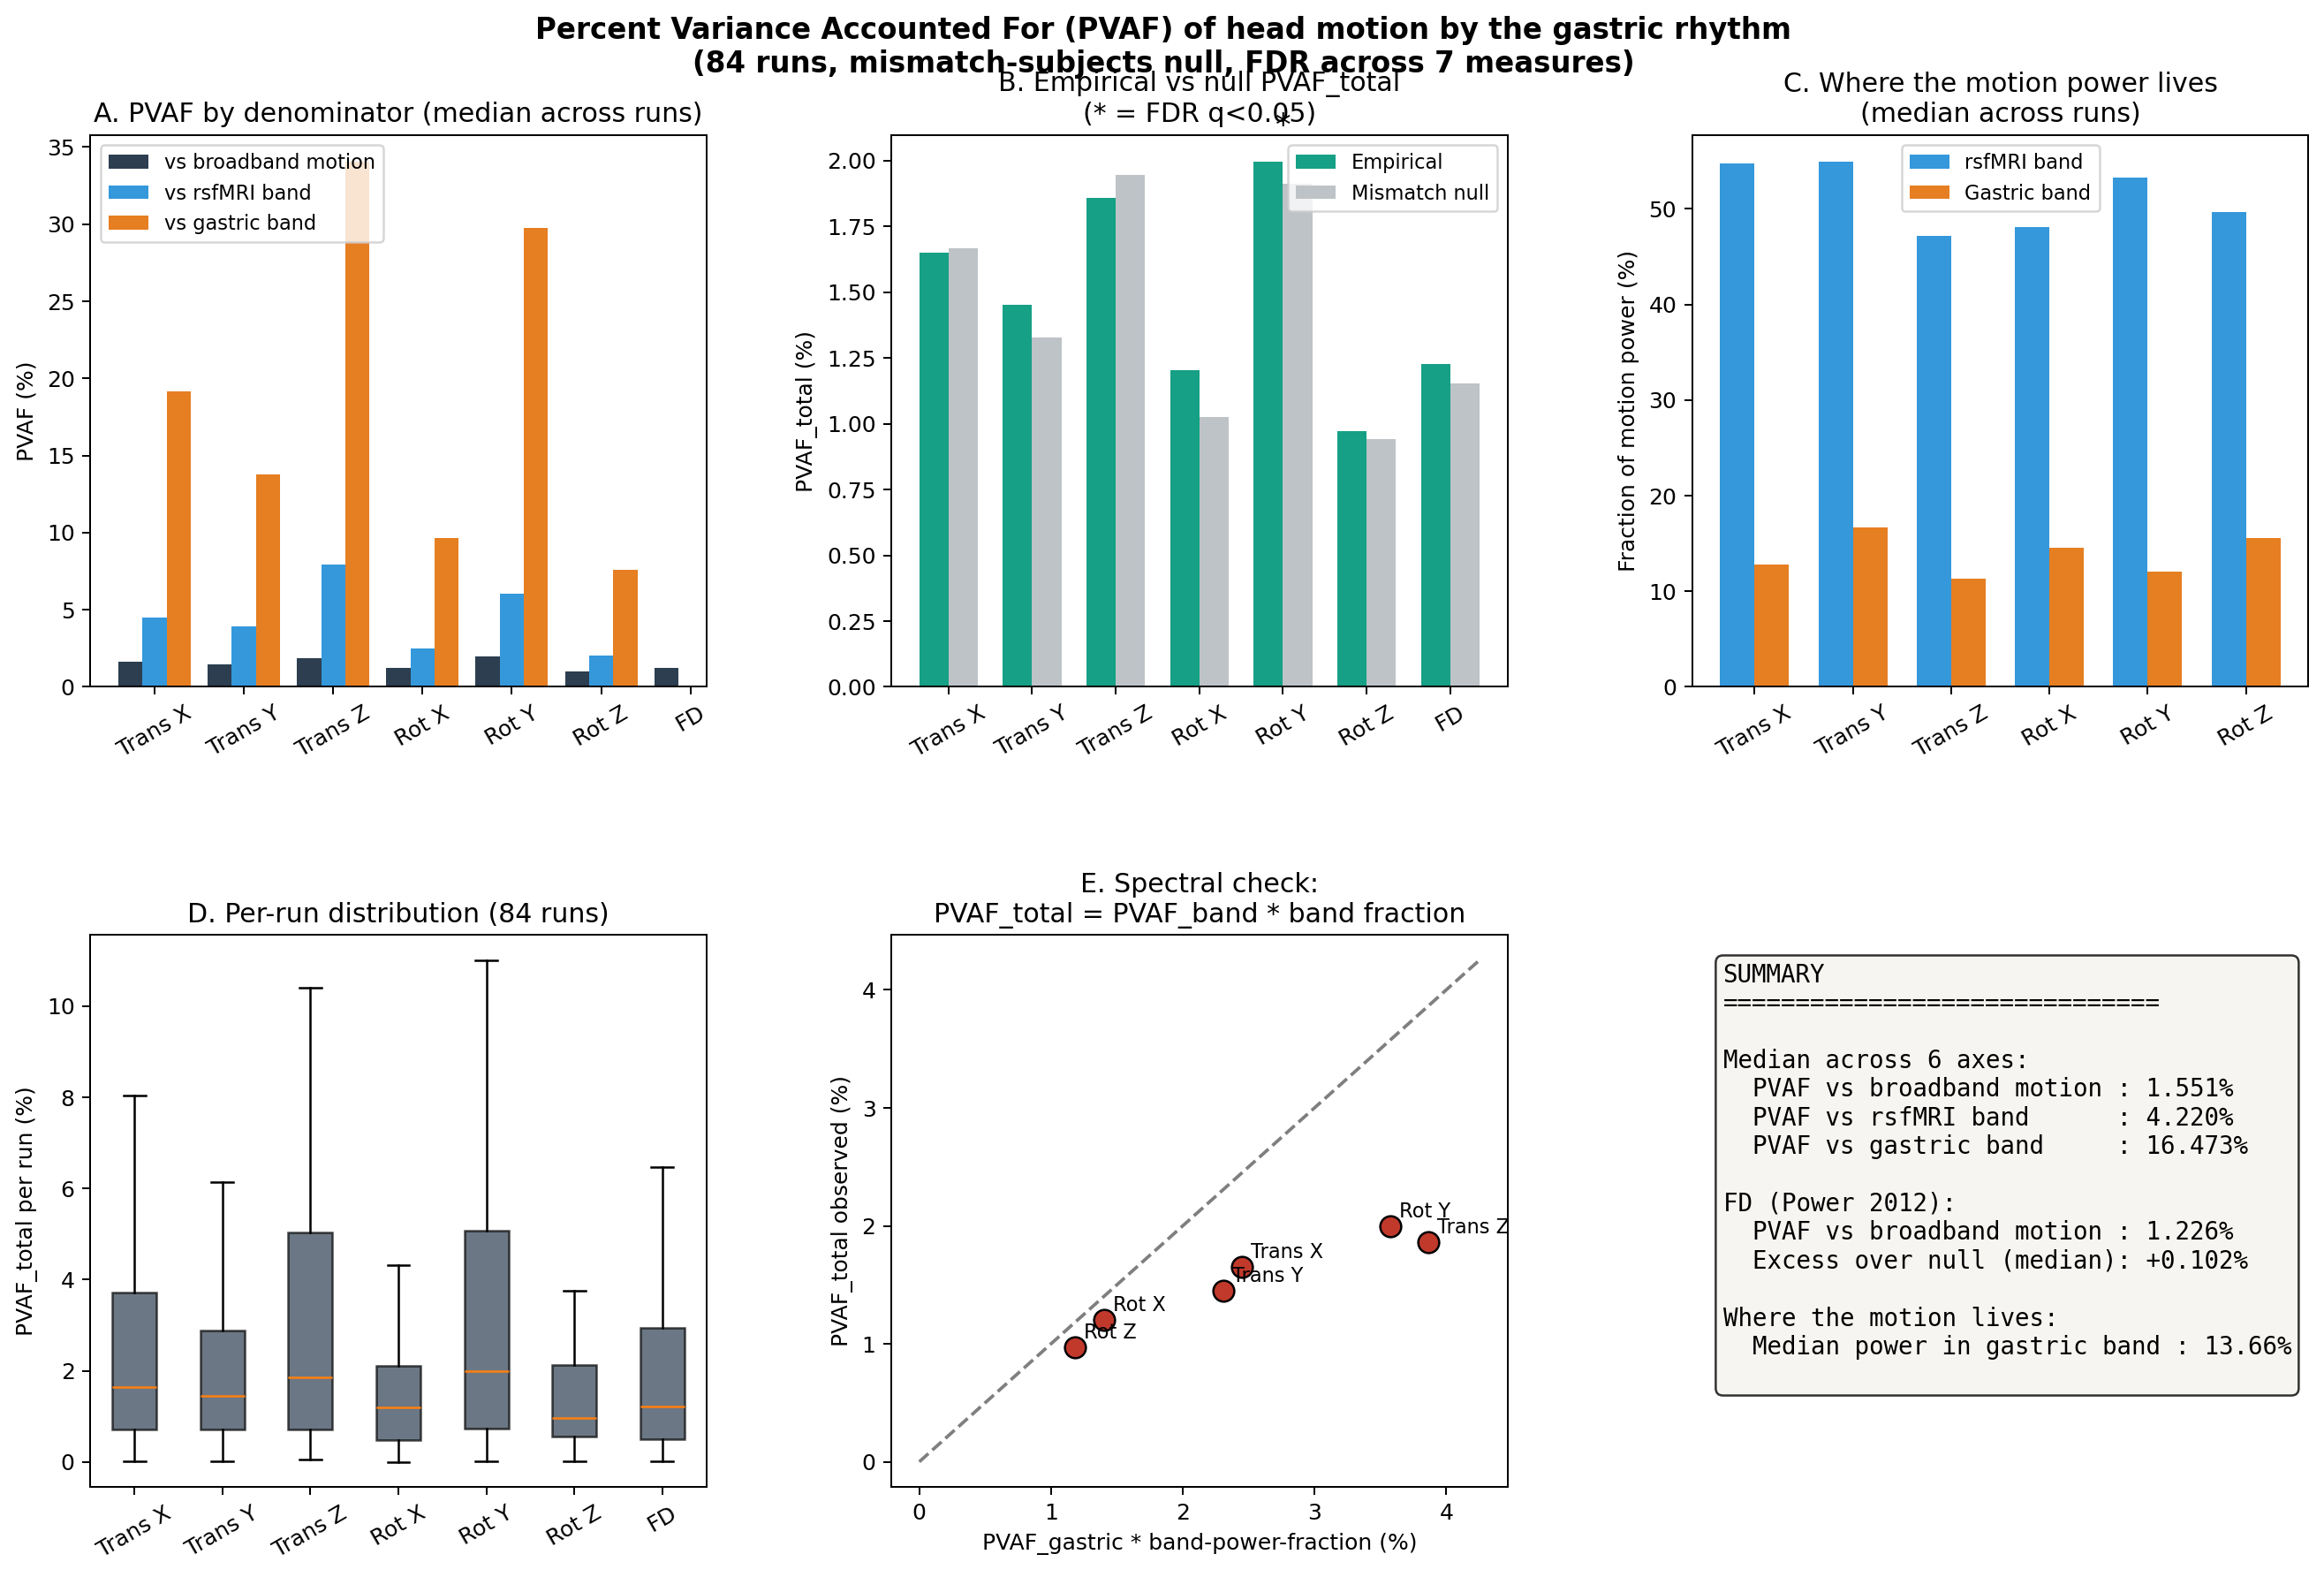
\includegraphics[width=0.98\linewidth]{outputs/pvaf_figure.png}
\caption{PVAF summary figure (six panels). A) PVAF per axis on the
three denominators; B) empirical vs.\ null $\PVAF_{\text{total}}$ with
FDR markers; C) fraction of motion power in each band per axis; D)
per-run distribution of $\PVAF_{\text{total}}$; E) spectral identity
check from equation~\ref{eq:identity}; F) numeric summary box.}
\label{fig:pvaf_summary}
\end{figure}

\section{Summary}

Based on thses results, across six head-motion parameters, the gastric rhythm linearly accounts
for a median of $1.5\%$ of total motion variance, and about $4.2\%$ of
motion variance in the rsfMRI band ($0.01$--$0.10$~Hz). The small
broadband number is driven primarily by the narrow gastric band holding
only $\sim 14\%$ of total motion power; within that band, the
regression recovers about $16\%$ of motion variance on average and
reaches $30$--$34\%$ for the two most coupled axes.

Framewise displacement is recovered at about $1.2\%$ of its total
variance, which appears consistent with the per-axis figures.

These numbers should be read with the caveat that they come from an
entirely linear regression of motion onto gastric phase and amplitude
on this dataset. They do not rule out larger non-linear or higher-order
coupling, and they do not speak to coupling that is amplitude-modulated
in a way that may average out under OLS. PLV and awPLV may be better
suited for those cases.

\section*{References}

\begin{itemize}
\item Birn RM \textit{et al.} (2006). Separating
respiratory-variation-related fluctuations from
neuronal-activity-related fluctuations in fMRI. \textit{NeuroImage}
31(4):1536--1548.
\item Brillinger DR (2001). \textit{Time Series: Data Analysis and
Theory.} SIAM.
\item Choe AS \textit{et al.} (2021). Phase-locking of resting-state
brain networks with the gastric basal electrical rhythm. \textit{PLoS
ONE} 16(1):e0244756.
\item Fisher NI (1993). \textit{Statistical Analysis of Circular Data.}
Cambridge University Press.
\item Levakov G, Ganor S, Avidan G (2023). Reliability and validity of
brain--gastric phase synchronization. \textit{Human Brain Mapping}
44:4956--4966.
\item Power JD \textit{et al.} (2012). Spurious but systematic
correlations in functional connectivity MRI networks arise from subject
motion. \textit{NeuroImage} 59(3):2142--2154.
\item Rebollo I \textit{et al.} (2018). Stomach-brain synchrony reveals
a novel, delayed-connectivity resting-state network in humans.
\textit{eLife} 7:e33321.
\item Welch PD (1967). The use of fast Fourier transform for the
estimation of power spectra: a method based on time averaging over
short, modified periodograms. \textit{IEEE Trans Audio Electroacoust}
15:70--73.
\end{itemize}

\end{document}
